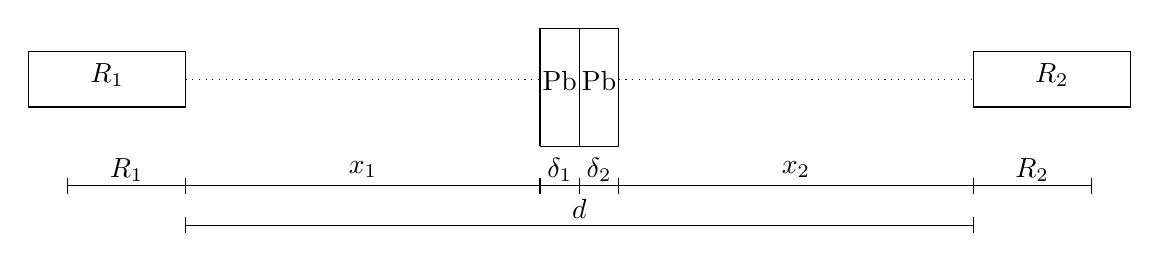
\begin{tikzpicture}
%\draw[->,thick] (-4,0)--(4,0) node[right]{$z$};

%\node [label=below:-e,draw,fill=black,circle,inner sep=0pt,minimum size=3pt] at (-3,0) {};
%\node [label=below:+e,draw,fill=black,circle,inner sep=0pt,minimum size=3pt] at (-2,0) {};
%\node [label=below:+e,draw,fill=black,circle,inner sep=0pt,minimum size=3pt] at (2,0) {};
%\node [label=below:-e,draw,fill=black,circle,inner sep=0pt,minimum size=3pt] at (3,0) {};


\draw[] (-4,0)--(-4,0.7)--(-2,0.7)--(-2,0)--(-4,0) node[label=above:$R_1$, black, midway, yshift=0.3]{}; %primo rivelatore
\draw[] (8,0)--(8,0.7)--(10,0.7)--(10,0)--(8,0) node[label=above:$R_2$, black, midway, yshift=0.3]{}; %secondo rivelatore

\draw[] (2.5,-0.5)--(2.5,1)--(3,1)--(3,-0.5)--(2.5,-0.5) node[label=above:Pb, black, midway, yshift=13]{}; %primo piombo
\draw[] (3,-0.5)--(3,1)--(3.5,1)--(3.5,-0.5)--(3,-0.5) node[label=above:Pb, black, midway, yshift=13]{}; %secondo piombo

%\node[starburst, minimum width=3cm, minimum height=2cm,line width=1.5pt]{};

\draw[] (-3.5,-1)--(9.5,-1) node[right]{};

\draw[] (-3.5,-1.1)--(-3.5,-0.9){};
\draw[] (-2,-1.1)--(-2,-0.9){};
\draw[] (2.5,-1.1)--(2.5,-0.9){};
\draw[] (3,-1.1)--(3,-0.9){};
\draw[] (3.5,-1.1)--(3.5,-0.9){};
\draw[] (8,-1.1)--(8,-0.9){};
\draw[] (9.5,-1.1)--(9.5,-0.9){};

\node[] at (-2.75,-0.8) {$R_1$};
\node[] at (0.25,-0.8) {$x_1$};
\node[] at (2.75,-0.8) {$\delta_1$};
\node[] at (3.25,-0.8) {$\delta_2$};
\node[] at (5.75,-0.8) {$x_2$};
\node[] at (8.75,-0.8) {$R_2$};

\draw[dotted](-2,0.35)--(2.5,0.35){};
\draw[dotted](3.5,0.35)--(8,0.35){};

\draw[] (-2,-1.5)--(8,-1.5) node[right]{};
\node[] at (3,-1.3) {$d$};
\draw[] (-2,-1.6)--(-2,-1.4){};
\draw[] (8,-1.6)--(8,-1.4){};


%\draw [decorate,decoration={brace,amplitude=10pt},xshift=0pt,yshift=0pt] (-3,0) -- (-2,0) node [label=above:$z_2$,black,midway,yshift=0.2cm] {};
%\draw [decorate,decoration={brace,amplitude=10pt},xshift=0pt,yshift=0pt] (-2,0) -- (2,0) node [label=above:$R$,black,midway,yshift=0.2cm] {};
%\draw [decorate,decoration={brace,amplitude=10pt},xshift=0pt,yshift=0pt] (2,0) -- (3,0) node [label=above:$z_1$,black,midway,yshift=0.2cm] {};

\end{tikzpicture} 
